\subsection{Effect of Cache Partitioning}

%% \begin{figure}[h]
%%   \centering
%%   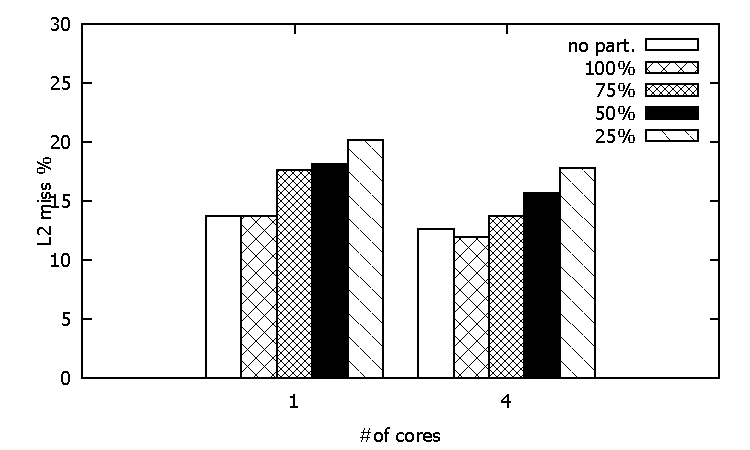
\includegraphics[width=.7\textwidth]{figs/palloc_multicore_l2missrate}
%%   \caption{L2 miss rate impact of limiting the amount of L2 cache space
%%   available to the DNN.}
%%   \label{fig:palloc_multicore_l2missrate}
%% \end{figure}

%% \begin{figure}[h]
%%   \centering
%%   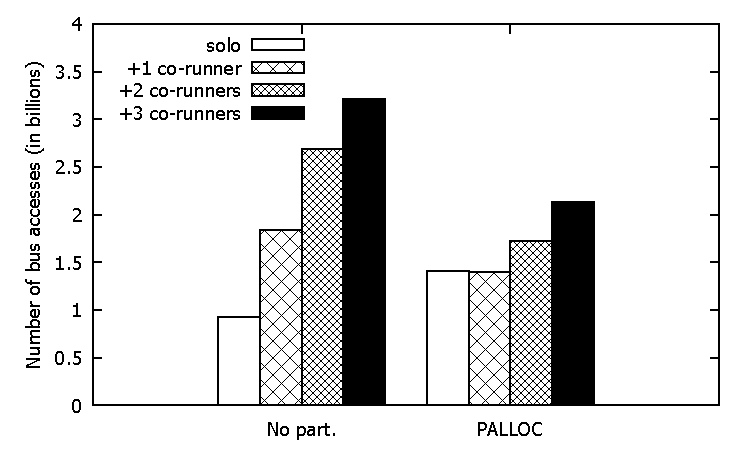
\includegraphics[width=.7\textwidth]{figs/palloc_bandwidth_modelbus}
%%   \caption{Model bus access impact of co-scheduling memory intensive co-runners 
%% when cache partitioning is enabled.}
%%   \label{fig:palloc_bandwidth_modelbus}
%% \end{figure}

%% \begin{figure}[h]
%%   \centering
%%   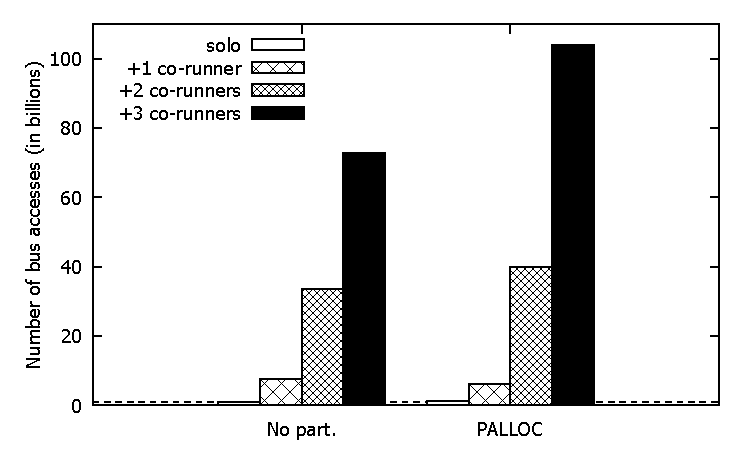
\includegraphics[width=.7\textwidth]{figs/palloc_bandwidth_bus}
%%   \caption{Total bus access impact of co-scheduling memory intensive co-runners 
%% when cache partitioning is enabled.}
%%   \label{fig:palloc_bandwidth_bus}
%% \end{figure}

%% \begin{figure}[h]
%%   \centering
%%   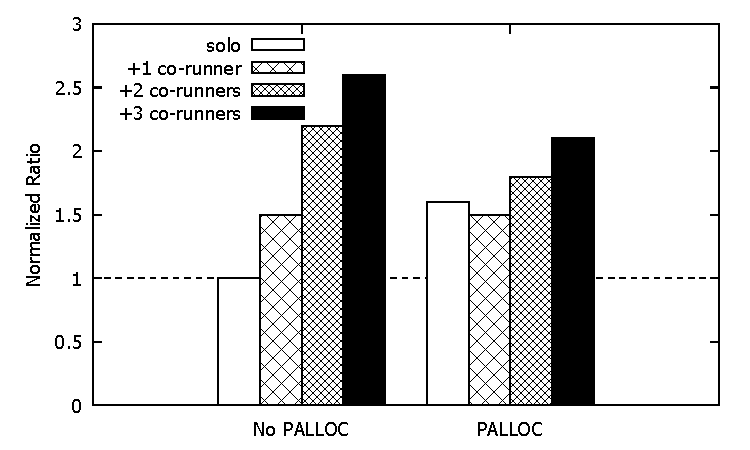
\includegraphics[width=.7\textwidth]{figs/palloc_bandwidth_l2missrate}
%%   \caption{L2 miss rate impact of co-scheduling memory intensive co-
%% runners when cache partitioning is enabled.}
%%   \label{fig:palloc_bandwidth_l2missrate}
%% \end{figure}

Cache partitioning is a well-known technique to improve isolation in
multicore systems by giving a dedicated cache space to each individaul 
task or core. In this experiment, we use PALLOC~\cite{yun2014rtas}, a
page-coloring based kernel-level memory allocator for Linux.
Page coloring is a OS technique that controls the physical addresses
of memory pages. By allocating pages over non-overlapping cache sets,
the OS can effectively partition the cache.
Using PALLOC, we investigate the effect of cache partitioning on
protecting DeepPicar's CNN based controller.

\begin{figure} [h]
  \centering
  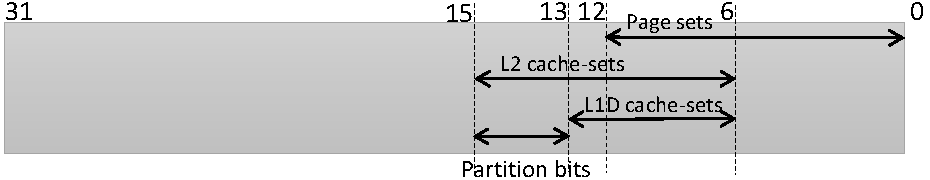
\includegraphics[width=.5\textwidth]{figs/cache-mapping}
  \caption{Physical address mapping of L1/L2 caches of Broadcom
    BCM2837 processor in Raspberry Pi 3.}
  \label{fig:cache-mapping}
\end{figure}

Figure~\ref{fig:cache-mapping} shows the physical address
mapping of the Raspberry Pi 3's BCM2837 processor, which has 32K private
L1 I\&D (4way) caches and a shared 512KB L2 (16 way) cache. In order
to avoid partitioning the private L1 caches, we use bits 13 and 14 for
coloring, which results in 4 usuable page colors.

%% determine if the DNN is mostly affected by the DRAM 
%% controller, we partition the L2 cache of the Pi3 and reperform the 
%% same experiments to see if there are any noticable changes. For the 
%% partition, we employ PALLOC~\cite{yun2014rtas}, a color-based page 
%% allocator that works on the kernel level.

%% For the bit mask, we select 
%% bits 12, 13 and 14 as they can be used to access the L2 cache,
%% as can be seen by Figure \ref{fig:cache-mapping}.
%% This results in 
%% 2\textsuperscript{3} = 8 colors, which we then assign to the Pi3's 
%% physical cores such that each core has two unique colors (colors 0 
%% and 1 are assigned to core 0, colors 2 and 3 are assigned to core 1, 
%% etc.). In the case of bit 12, since we use 2 colors for each partition,
%% the L1 Data cache is not partitioned in our experiments.

In the first experiment, we investigate the cache space sensitivity of
the DeepPicar's CNN-based control loop. Using PALLOC, we create 4
different cgroups which are configured to use 4, 3,
2, and 1 colors (100\%, 75\%, 50\% and 25\% of the L2 cache
space, respectively). We then execute the CNN control loop (inference)
on one core using a different cgroup cache partition, one at a time,
and measure the average processing time.

\begin{figure}[h]
  \centering
  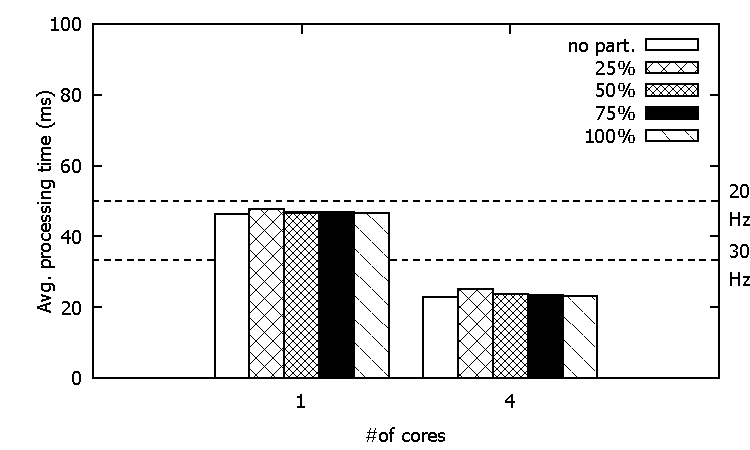
\includegraphics[width=.45\textwidth]{figs/palloc_multicore}
  \caption{Cache space sensitivity of the CNN controller.}
  \label{fig:palloc_multicore}
\end{figure}

Figure~\ref{fig:palloc_multicore} shows the results. As can be seen,
the CNN inference timing hardly changes at all regardless of the
size of the allocated L2 cache space. In other words, we find that
the CNN workload is largely insensitive to L2 cache space.

The next experiment further validates this finding. In this
experiment, we repeat the experiment in
Section~\ref{sec:eval-memhog}---i.e., co-scheduling the CNN model and
three Bandwidth (BwRead or BwWrite) instances---but this time we
ensure that each task is given equal amounts of L2 cache space by
assigning one color to each task's cache partition.

\begin{figure}[h]
  \centering
  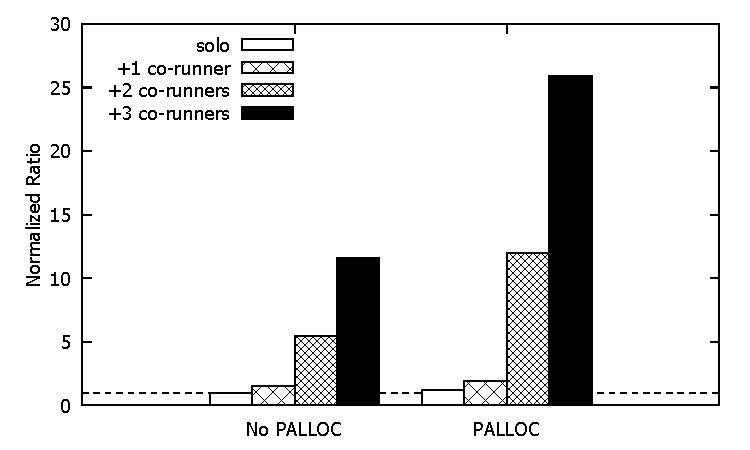
\includegraphics[width=.45\textwidth]{figs/palloc_bandwidth_exectime}
  \caption{Average processing time vs. the number of memory
intensive co-runners; Each core (task) is given a equal-sized
dedicated cache partition.}
  \label{fig:palloc_bandwidth_exectime}
\end{figure}

Figure \ref{fig:palloc_bandwidth_exectime} shows the
results. Compared to Figure~\ref{fig:perf_vs_bandwidth} where no cache
partioning is applied, assigning a dedicated L2 cache parititon to
each core does not provide significant isolation benefits. For BwRead
co-runners, cache partitioning slightly improves isolation, but for
BwWrite co-runners, cache partitioning causes worse worst-case
slowdown.

In summary, we find that the CNN inferencing workload is not sensitive
to cache space and that cache partitioning is not effective in
providing timing isolation for our CNN workload.

%% By partitioning the shared L2 cache, we find that no noticable 
%% improvements are gained and that performance remains consistent. 
%% In all experiements, the model shows no sensitivity to the shared L2 
%% cache. As a result, we conclude that cache partitioning is not an 
%% effective isolation mechanism, and that the performance of the shared 
%% DRAM controller is of greater importance to the real-time efficiacy of 
%% the DeepPicar.

%% If performance improves as a result of partitioning the shared cache 
%% then we know that the DNN, to some extent, relies on the shared cache 
%% in addition to the shared DRAM. On the other 
%% hand, if there is no improvement in performance, then it can be 
%% observed that the shared memory is more critical for the DNN.

%% We run the DNN model with different amounts of L2 cache being
%% available based on the number of colors being used. For example, if two 
%% colors are used, then 25\% of the L2 cache is available, whereas if all 
%% 8 colors are used, 100\% of the L2 cache is available. Particularly, we 
%% test the performance of the model when it utilizes a single core and
%% all four of the available cores. 

%% As expected, the amount of L2 cache 
%% available to the model does not result in any significant changes in 
%% performance. 
%% This can also be seen by the L2 miss rates of the model 
%% seen in \ref{fig:palloc_multicore_l2missrate}. As more cache space 
%% becomes avaiable, the percentage of L2 misses decreases, which doesn't 
%% affect the real-time performance of the DNN. As such, we find that a 
%% single model is not sensitive to the shared L2 cache.

%% \begin{figure}[h]
%%  \centering
%%   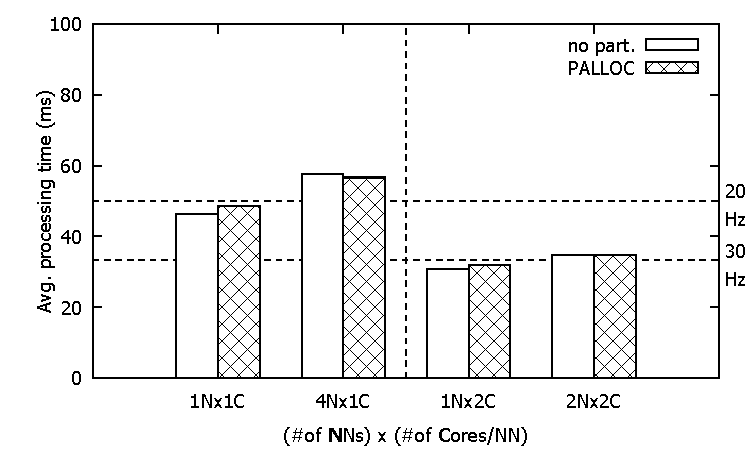
\includegraphics[width=.45\textwidth]{figs/palloc_multimodel}
%%   \caption{Timing impact of co-scheduling multiple DNNs when cache 
%% partitioning is enabled.}
%%   \label{fig:palloc_multimodel}
%% \end{figure}

%% We also co-schedule multiple models to see how cache partitioning affects
%% interference between them. Each model uses an equal number of colors, and
%% are thus given equal amounts of L2 cache space, and there is no overlap
%% in the colors used, so no L2 cache is shared between models. As can be 
%% seen in Figure \ref{fig:palloc_multimodel}, the performance of the models 
%% remains the same as when no cache partitioning was employed. Based of 
%% these results, we find that contention for the L2 cache is not the main
%% source of interference between multiple DNN models.

%% At the same time, though, the L2 miss rates of the model don't correlate 
%% to the timing increases seen, as is shown in 
%% \ref{fig:palloc_bandwidth_l2missrate}. Instead, we find that the number
%% of bus accesses increases when cache partitions are used, and they mirror
%% the timing increases of the model. This can be seen in Figure 
%% \ref{fig:palloc_bandwidth_bus}. These additional bus accesses are
%% most likely caused by the L2 prefetcher, as it can generate additional bus
%% accesses that aren't counted as L2 misses. As a result, we find that cache
%% partitioning is detrimental to the performance of the DNN so long as the 
%% 0L2 prefetcher is enabled (we have not yet found a way to disable it on
%% the Pi 3). Furthermore, no cache sensitivity was displayed by the model,
%% thus showing that the performance of the L2 cache is not vital for DNN 
%% performance when co-runners are introduced.

